% ============================================================================
% ECOI2217 - Inteligencia Artificial - Atividade N2: Algoritmos Geneticos
% Baseado no template IEEE (IWSSIP) fornecido na disciplina.
% Compilar: pdflatex main && bibtex main && pdflatex main && pdflatex main
%           (ou: latexmk -pdf main.tex). Compativel com Overleaf.
% As tabelas em tables/ e as figuras em figures/ sao geradas por executar_tudo.py.
% ============================================================================
\documentclass[conference]{IEEEtran}
\IEEEoverridecommandlockouts
\usepackage[utf8]{inputenc}
\usepackage[T1]{fontenc}
\usepackage[brazil]{babel}
\usepackage{cite}
\usepackage{amsmath,amssymb,amsfonts}
\usepackage{graphicx}
\usepackage{textcomp}
\usepackage{xcolor}
\usepackage{booktabs}
\usepackage{url}
\usepackage[ruled,vlined,linesnumbered,portuguese]{algorithm2e}
\usepackage{listings}
\usepackage[hidelinks]{hyperref}
\usepackage{flushend} % equilibra as colunas da última página (como no template)
\usepackage[a4paper, left=0.51in, right=0.51in, top=0.75in, bottom=1.69in]{geometry} % margens do template fornecido

\graphicspath{{figures/}}

% ---------------------------------------------------------------- listings --
\renewcommand{\lstlistingname}{Listagem}
\lstdefinestyle{py}{
  language=Python,
  basicstyle=\ttfamily\scriptsize,
  keywordstyle=\color{blue!55!black}\bfseries,
  commentstyle=\color{black!55}\itshape,
  stringstyle=\color{orange!70!black},
  showstringspaces=false,
  frame=tb, framerule=0.4pt,
  breaklines=true, columns=fullflexible, keepspaces=true,
  aboveskip=4pt, belowskip=2pt, xleftmargin=1pt,
  literate={á}{{\'a}}1 {à}{{\`a}}1 {ã}{{\~a}}1 {â}{{\^a}}1 {é}{{\'e}}1 {ê}{{\^e}}1
           {í}{{\'i}}1 {ó}{{\'o}}1 {õ}{{\~o}}1 {ô}{{\^o}}1 {ú}{{\'u}}1 {ç}{{\c{c}}}1
}
\lstset{style=py}

\newcommand{\deap}{\textsc{DEAP}}
\newcommand{\code}[1]{\texttt{#1}}

\begin{document}

\title{Algoritmos Evolucionários}

\author{\IEEEauthorblockN{Kleber Augusto Barbosa}
\IEEEauthorblockA{Engenharia de Computação -- ECOI2217 Inteligência Artificial\\
Universidade Federal de Itajubá -- Itabira, MG, Brasil\\
kleberbarbosa@unifei.edu.br}}

\maketitle

\begin{abstract}
Este trabalho aplica Algoritmos Genéticos (AG) a dois problemas. No primeiro, implementado sem bibliotecas de AG, escolhem-se os voos de ida e volta de seis pesquisadores para um congresso em Roma, buscando o menor custo de passagens e o menor tempo de espera no aeroporto. Cada indivíduo é um vetor de 12 índices que apontam para voos reais do arquivo de dados, e a fitness soma o custo e a espera. O AG encontrou a melhor solução possível em 25 de 30 execuções sem restrição de horário e em todas as 30 com a janela de uma mesa-redonda. No segundo problema, a função de Rastrigin é minimizada com a biblioteca \deap{} para $n=2$ e $n=10$, e em todas as execuções o AG chegou à região do mínimo global. O trabalho inclui também um breve tutorial da \deap{}.
\end{abstract}

\renewcommand\IEEEkeywordsname{Palavras-chave}
\begin{IEEEkeywords}
Algoritmos Genéticos, otimização combinatória, função de Rastrigin, DEAP, seleção por torneio, elitismo.
\end{IEEEkeywords}

% ============================================================================
\section{Introdução}
% ============================================================================
Algoritmos Genéticos são métodos de busca estocástica inspirados na seleção natural~\cite{goldberg1989}. Eles mantêm uma população de soluções candidatas (indivíduos), avaliam cada uma por uma função de aptidão (\emph{fitness}) e geram novas soluções por seleção, cruzamento e mutação. Não exigem gradiente nem convexidade e se aplicam tanto a espaços discretos e combinatórios quanto a funções contínuas multimodais.

Este trabalho resolve as duas atividades da avaliação N2 da disciplina ECOI2217:
\begin{enumerate}
  \item \textbf{Atividade 1:} escolher, entre os 120 voos de \code{flights.txt}, as passagens de ida e volta de seis pesquisadores (Lisboa, Madri, Paris, Dublin, Bruxelas e Londres) para um congresso em Roma, com o menor preço e o menor tempo de espera nos aeroportos. O problema segue o exemplo clássico de otimização de viagens em grupo de Segaran~\cite{segaran2007}. O AG foi implementado \textbf{sem bibliotecas de AG}.
  \item \textbf{Atividade 2:} minimizar a função de Rastrigin~\cite{surjanovic2013} para $n=2$ e $n=10$, usando a biblioteca \deap{}~\cite{fortin2012deap}.
\end{enumerate}

As contribuições do trabalho são:
\begin{itemize}
  \item a formalização das premissas de horário da Atividade 1, incluindo um cenário com janela fixa para a mesa-redonda;
  \item uma validação do AG contra o ótimo global \emph{exato}, viabilizada pela separabilidade da fitness;
  \item uma análise estatística (média, variância e desvio padrão em 30 execuções) com comparação contra busca aleatória de mesmo orçamento e análise de sensibilidade dos parâmetros;
  \item um tutorial de \deap{}.
\end{itemize}
O código é reprodutível por \emph{seed} e acompanha este documento.

% ============================================================================
\section{Fundamentação: componentes do AG}
\label{sec:ga}
% ============================================================================
Um AG geracional repete o seguinte ciclo:
\begin{enumerate}
  \item avaliar a população $\mathcal{P}_t$;
  \item selecionar pais;
  \item recombiná-los com probabilidade $p_c$;
  \item mutar os filhos com probabilidade $p_m$;
  \item formar $\mathcal{P}_{t+1}$.
\end{enumerate}

\textbf{Representação.} É a escolha do cromossomo. Ela define o espaço que o AG realmente explora e quais operadores produzem descendentes válidos.

\textbf{Seleção por torneio.} Sorteiam-se $k$ indivíduos e o de melhor fitness vence. O parâmetro $k$ controla a pressão seletiva: com $k$ maior, os bons indivíduos dominam mais rápido, com risco de convergência prematura. O torneio depende só da ordem das fitness, e não da escala, o que é útil quando a fitness inclui penalidades de magnitude muito diferente.

\textbf{Elitismo.} Os $e$ melhores indivíduos são copiados sem alteração para a próxima geração. Isso garante que a melhor fitness da população nunca piora.

% ============================================================================
\section{Atividade 1: voos para o congresso em Roma}
\label{sec:a1}
% ============================================================================
\subsection{Dados e espaço de busca}
O arquivo \code{flights.txt} tem 120 linhas no formato \code{ORIGEM,DESTINO,PARTIDA,CHEGADA,PREÇO}, por exemplo \code{MAD,FCO,11:01,12:39,260}. Para cada uma das seis cidades há 10 voos de ida (origem$\to$FCO) e 10 voos de volta (FCO$\to$origem). Os horários foram convertidos para minutos desde 00:00, e cada lista de voos foi ordenada por horário de partida. O espaço de busca tem $10^{12}$ combinações.

\subsection{Premissas adotadas}
\label{sec:a1_premissas}
O enunciado diz que os pesquisadores pegam \emph{uma van} no aeroporto até o congresso e voltam na mesma van. Disso decorrem as premissas abaixo, com $\tau_t=45$~min de translado FCO$\leftrightarrow$congresso e $\tau_c=60$~min de antecedência mínima para o check-in:
\begin{enumerate}
\item[P1)] A van só parte de FCO quando o \textbf{último} pesquisador chega. Quem chega antes espera.
\item[P2)] Na volta, a van deixa todos juntos em FCO, no instante $t_{\text{drop}}$. Cada pesquisador espera até a partida do próprio voo.
\item[P3)] \textbf{Cenário A} (ida e volta em dias distintos, como no problema original): não há janela. A van chega a FCO $\tau_c$ minutos antes do primeiro voo de volta.
\item[P4)] \textbf{Cenário B} (mesa-redonda das 14:00 às 16:00 no mesmo dia da viagem): o grupo deve chegar ao congresso até o início da mesa ($t_{\text{van}}+\tau_t\le$ 14:00). A van sai do congresso às 16:00, então $t_{\text{drop}}=$ 16:45, e todo voo de volta deve partir após $t_{\text{drop}}+\tau_c=$ 17:45.
\item[P5)] Nenhum voo cruza a meia-noite (verificado na leitura dos dados). O tempo gasto dentro do avião não é espera. Só conta o tempo parado no aeroporto de Roma.
\end{enumerate}

\subsection{Representação do indivíduo}
O cromossomo é um vetor de 12 inteiros, com dois genes por pesquisador:
\begin{equation}
\mathbf{x}=(o_1,r_1,\;o_2,r_2,\;\dots,\;o_6,r_6),\qquad o_i,r_i\in\{0,\dots,9\},
\end{equation}
em que $o_i$ indexa o voo de ida e $r_i$ o voo de volta do pesquisador $i$, nesta ordem: LIS, MAD, CDG, DUB, BRU, LHR. Por exemplo, $o_2=4$ é o quinto voo MAD$\to$FCO do dia (12:44--14:17, 134~EUR). A representação tem três consequências diretas:
\begin{itemize}
  \item \textbf{Fitness:} decodificar é uma consulta em tabela ($O_i[o_i]$, $R_i[r_i]$), o que permite avaliar a população inteira de forma vetorizada.
  \item \textbf{Cruzamento:} como todo locus tem o mesmo domínio em qualquer indivíduo, trocar genes da mesma posição sempre gera um filho válido.
  \item \textbf{Mutação:} basta sortear outro índice em $\{0,\dots,9\}$. Por causa da ordenação por horário, somar $\pm1$ ao gene equivale a escolher o voo imediatamente anterior ou posterior da mesma rota.
\end{itemize}
Nenhum operador consegue, portanto, criar voos inexistentes.

\subsection{Função fitness}
Sejam $a_i$ o horário de chegada do voo de ida, $d_i$ o horário de partida do voo de volta e $c(\cdot)$ o preço de um voo. O custo total é
\begin{equation}
C(\mathbf{x})=\sum_{i=1}^{6}\big[c(O_i[o_i])+c(R_i[r_i])\big].
\end{equation}
Pela premissa P1, a van parte em $t_{\text{van}}=\max_i a_i$. Pela premissa P2, o grupo é deixado em FCO em
\begin{equation}
t_{\text{drop}}=\begin{cases}\min_i d_i-\tau_c, & \text{cenário A}\\ t_{\text{fim}}+\tau_t, & \text{cenário B.}\end{cases}
\end{equation}
A espera total, em minutos, é
\begin{equation}
W(\mathbf{x})=\sum_{i=1}^{6}(t_{\text{van}}-a_i)\;+\;\sum_{i=1}^{6}\max(0,\,d_i-t_{\text{drop}}).
\end{equation}
No cenário B, as violações (em minutos) são
\begin{equation}
g_0=\max(0,\;t_{\text{van}}+\tau_t-t_{\text{ini}}),\quad
g_i=\max(0,\;t_{\text{drop}}+\tau_c-d_i).
\end{equation}
Elas entram em uma penalidade com uma parcela fixa e outra proporcional:
\begin{equation}
P(\mathbf{x})=\rho_f\sum_{j=0}^{6}[g_j>0]\;+\;\rho_m\sum_{j=0}^{6}g_j,
\end{equation}
com $\rho_f=1000$~EUR por restrição violada e $\rho_m=10$~EUR/min. A parcela proporcional diferencia soluções \emph{quase} factíveis das muito infactíveis e assim guia a busca para a região factível. No cenário B, só $1{,}3\times10^{-3}$ das combinações de ida e $6{,}4\times10^{-5}$ das de volta são factíveis. A fitness a ser \textbf{minimizada} é
\begin{equation}
F(\mathbf{x})=C(\mathbf{x})+\lambda\,W(\mathbf{x})+P(\mathbf{x}),
\label{eq:fitness}
\end{equation}
em que $\lambda$ (EUR/min) é o custo atribuído a um minuto de espera. Usou-se $\lambda=1$, isto é, 60~EUR por hora parada, que deixa custo e espera na mesma ordem de grandeza. A Seção~\ref{sec:res_a1} varia $\lambda$ para traçar o compromisso entre os dois objetivos.

\subsection{Operadores genéticos}
\begin{itemize}
\item \textbf{Inicialização:} cada gene é sorteado uniformemente em $\{0,\dots,9\}$.
\item \textbf{Seleção:} torneio determinístico de tamanho $k=3$, com reposição.
\item \textbf{Cruzamento uniforme:} com probabilidade $p_c$, cada locus do par de pais é trocado com probabilidade $1/2$, gerando dois filhos. As variantes de 1 e 2 pontos também foram implementadas.
\item \textbf{Mutação por gene:} cada gene muta com probabilidade $p_m$. Metade das mutações é do tipo \emph{creep} ($\pm1$, refletido nas bordas), um ajuste fino de horário. A outra metade é \emph{reset}: sorteia-se outro voo da rota, sempre diferente do atual.
\item \textbf{Mutação de bloco:} com probabilidade $p_{\text{shift}}$, um filho tem \emph{todos} os genes de ida, ou todos os de volta, deslocados pelo mesmo passo $\pm1$.
\end{itemize}

A mutação de bloco foi introduzida depois de observar a estagnação do AG. A fitness acopla os seis pesquisadores por $\max_i a_i$ e $\min_i d_i$. Uma solução boa é, por isso, um \emph{grupo sincronizado}: todos chegam perto do mesmo horário e todos partem perto do mesmo horário. Mudar um único voo desse grupo quase sempre aumenta a espera de todos. Assim, os ótimos locais são agrupamentos em outros horários do dia, e a mutação gene a gene raramente sai deles. Deslocar o bloco inteiro mantém a sincronia e move o grupo para o horário vizinho. O operador explora a ordenação temporal da representação e só produz índices válidos.

O elitismo copia os $e=5$ melhores indivíduos. O laço completo está no Algoritmo~\ref{alg:a1}. Todas as operações sobre a população são vetorizadas com \code{numpy}.

\begin{algorithm}[!t]
\caption{AG da Atividade 1 (implementação própria)}
\label{alg:a1}
\small
\KwIn{$N$, $G$, $k$, $p_c$, $p_m$, $p_{\text{shift}}$, $e$, seed}
\KwOut{melhor cromossomo encontrado}
$\mathcal{P}\leftarrow N$ vetores com genes $\sim\mathcal{U}\{0..9\}$; avaliar $F(\mathcal{P})$\;
\For{$g\leftarrow1$ \KwTo $G$}{
  $\mathcal{E}\leftarrow$ os $e$ melhores de $\mathcal{P}$ (sem reavaliação)\;
  selecionar $N-e$ pais por torneio de tamanho $k$\;
  \ForEach{par de pais $(p_1,p_2)$}{
    \lIf{$\mathcal{U}(0,1)<p_c$}{$(f_1,f_2)\leftarrow$ cruzamento uniforme}
    \lElse{$(f_1,f_2)\leftarrow(p_1,p_2)$}
  }
  mutar cada gene dos filhos com prob. $p_m$ (creep $\pm1$ ou reset)\;
  mutação de bloco em cada filho com prob. $p_{\text{shift}}$\;
  avaliar os filhos; $\mathcal{P}\leftarrow\mathcal{E}\cup$ filhos\;
  registrar $F$ melhor, médio e pior e a diversidade\;
}
\Return melhor indivíduo de $\mathcal{P}$\;
\end{algorithm}

\subsection{Validação pelo ótimo exato}
Enumerar $10^{12}$ soluções é inviável. Porém, pelas Eqs.~(3)--(7), a parte de ida de $F$ depende apenas de $(o_1,\dots,o_6)$ e a parte de volta apenas de $(r_1,\dots,r_6)$. Logo, $F=F_{\text{ida}}+F_{\text{volta}}$ e $\min F=\min F_{\text{ida}}+\min F_{\text{volta}}$. Basta enumerar $2\times10^6$ combinações, o que leva menos de 0,5~s com \code{numpy}. O ótimo exato $F^*$ é usado \emph{apenas} para avaliar o AG, por meio da taxa de execuções que o atingem e do \emph{gap} até ele. O AG não usa essa informação, pois a separabilidade é uma particularidade desta modelagem e não vale em geral. A mesma decomposição fornece a fronteira de Pareto exata entre custo e espera. Ela é obtida pela soma de Minkowski das fronteiras de ida e de volta, seguida de filtragem dos pontos dominados.

\subsection{Parâmetros}
A Tabela~\ref{tab:a1_params} lista os parâmetros. A configuração base foi escolhida em um ajuste preliminar com \emph{seeds} diferentes das usadas nos experimentos finais, para não ajustar os parâmetros às mesmas execuções que são reportadas.

\begin{table}[!t]
\centering
\footnotesize
\setlength{\tabcolsep}{4pt}
\caption{Parâmetros do AG da Atividade 1 (implementação própria).}
\label{tab:a1_params}
\begin{tabular}{@{}lp{4.6cm}@{}}
\toprule
Parâmetro & Valor \\
\midrule
Representação & 12 inteiros (ida/volta de cada pesquisador), gene $\in\{0..9\}$ \\
Tamanho da população $N$ & 150 \\
Número de gerações $G$ & 400 \\
Seleção & torneio determinístico, $k=3$, com reposição \\
Cruzamento & uniforme, $p_c=0{,}90$ \\
Mutação por gene & $p_m=0{,}05$ (50\% creep $\pm1$, resto reset) \\
Mutação de bloco & $p_{\mathrm{shift}}=0{,}30$ por filho \\
Elitismo & 5 melhores copiados sem alteração \\
Avaliações/execução & 58.150 \\
Execuções & 30 (seeds 2026--2055) \\
\midrule
$\lambda$ (custo da espera) & 1 EUR/min \\
Check-in / translado & 60 min / 45 min \\
Janela (cenário B) & 14:00--16:00 \\
Penalidade (cenário B) & 1.000 EUR/restrição + 10 EUR/min \\
\bottomrule
\end{tabular}
\end{table}


% ============================================================================
\section{Atividade 2: função de Rastrigin com DEAP}
\label{sec:a2}
% ============================================================================
\subsection{Definição}
\begin{equation}
f(\mathbf{x})=An+\sum_{i=1}^{n}\left[x_i^2-A\cos(2\pi x_i)\right],\quad A=10,
\end{equation}
com $x_i\in[-5{,}12;\,5{,}12]$ e mínimo global $f(\mathbf{0})=0$. Cada coordenada contribui com $x_i^2+A(1-\cos 2\pi x_i)\ge0$, termo que tem mínimos locais próximos de cada inteiro $k$, de valor $\approx k^2$. Assim, $f\approx m$ indica $m$ coordenadas presas em $\pm1$. Além disso, $f<0{,}5$ só ocorre se todo $|x_i|\lesssim0{,}05$, ou seja, se a solução está na bacia do ótimo global. Para $n=2$ existem cerca de 100 mínimos locais no domínio. Para $n=10$, o número cresce exponencialmente.

\subsection{Representação e operadores}
O cromossomo é uma lista de $n$ reais (\code{creator.Individuo}, que herda de \code{list}), e a fitness é o próprio $f$ com peso $-1$ (minimização). Como o domínio é uma caixa, foram usados operadores \emph{limitados}, que nunca geram genes fora de $[-5{,}12;\,5{,}12]$:
\begin{itemize}
\item \textbf{Cruzamento SBX}~\cite{deb1995sbx}: os filhos ficam a uma distância dos pais controlada pelo índice $\eta_c$. Com $\eta_c$ alto, os filhos ficam perto dos pais; com $\eta_c$ baixo, a busca é mais exploratória. O operador atua coordenada a coordenada, o que combina com a separabilidade da Rastrigin.
\item \textbf{Mutação polinomial}: perturba cada gene com probabilidade $p_{\text{gene}}=1/n$, com amplitude controlada por $\eta_m$.
\item \textbf{Seleção:} torneio com $k=3$.
\end{itemize}

\subsection{Elitismo no DEAP}
O algoritmo pronto \code{algorithms.eaSimple} não é elitista: o \code{HallOfFame} apenas \emph{armazena} o melhor indivíduo, sem devolvê-lo à população. Por isso foi escrito um laço geracional próprio (\code{ag\_elitista}, Listagem~\ref{lst:elit}). A cada geração, ele copia os $e=2$ melhores e completa a população com $N-e$ filhos gerados por \code{varAnd}. Estatísticas, \code{Logbook} e \code{HallOfFame} continuam sendo os da biblioteca. A Tabela~\ref{tab:a2_params} resume os parâmetros.

\begin{table}[!t]
\centering
\footnotesize
\setlength{\tabcolsep}{4pt}
\caption{Parâmetros do AG da Atividade 2 (DEAP); domínio $[-5{,}12;\,5{,}12]^n$, seeds 2026--2055.}
\label{tab:a2_params}
\begin{tabular}{@{}lcc@{}}
\toprule
Parâmetro & $n=2$ & $n=10$ \\
\midrule
Representação & 2 reais & 10 reais \\
População $N$ & 100 & 200 \\
Gerações $G$ & 100 & 500 \\
Seleção (torneio) & $k=3$ & $k=3$ \\
Cruzamento SBX: $p_c$ / $\eta_c$ & 0{,}9 / 15 & 0{,}9 / 15 \\
Mutação polinomial: $\eta_m$ & 20 & 20 \\
\quad prob. por indivíduo / gene & 1{,}0 / 0{,}50 & 1{,}0 / 0{,}10 \\
Elitismo & 2 melhores & 2 melhores \\
Avaliações/execução (máx.) & 9.900 & 99.200 \\
Execuções & 30 & 30 \\
\bottomrule
\end{tabular}
\end{table}


% ============================================================================
\section{Tutorial prático: DEAP em cinco passos}
\label{sec:tutorial}
% ============================================================================
O \deap{} (\emph{Distributed Evolutionary Algorithms in Python}) não impõe um algoritmo fechado. Ele fornece tipos, operadores e laços prontos, que o usuário combina por meio de uma \emph{caixa de ferramentas} (\code{Toolbox}). Para instalar:
\begin{lstlisting}[language=bash,numbers=none]
pip install deap numpy
\end{lstlisting}

\textbf{Passo 1 -- Tipos com \code{creator}.} O \code{creator.create} gera classes em tempo de execução. Aqui, uma \code{Fitness} com pesos (sinal $-1$ para minimizar, $+1$ para maximizar; uma tupla com vários pesos define um problema multiobjetivo) e um \code{Individuo} que é uma \code{list} com um atributo \code{fitness}.
\begin{lstlisting}
import random
from deap import base, creator, tools, algorithms

creator.create("FitnessMin", base.Fitness, weights=(-1.0,))
creator.create("Individuo", list, fitness=creator.FitnessMin)
\end{lstlisting}

\textbf{Passo 2 -- \code{base.Toolbox} e inicialização.} O método \code{register(alias, função, *args)} guarda uma função com argumentos pré-fixados (equivale a \code{functools.partial}). O \code{tools.initRepeat} chama o gerador $n$ vezes e embala o resultado no contêiner indicado.
\begin{lstlisting}
LIM_INF, LIM_SUP, N = -5.12, 5.12, 10
tb = base.Toolbox()
tb.register("gene", random.uniform, LIM_INF, LIM_SUP)
tb.register("individuo", tools.initRepeat,
            creator.Individuo, tb.gene, n=N)
tb.register("populacao", tools.initRepeat, list, tb.individuo)
pop = tb.populacao(n=200)
\end{lstlisting}

\textbf{Passo 3 -- Avaliação e operadores.} A função de avaliação \textbf{deve devolver uma tupla}, mesmo com um único objetivo. Os nomes \code{mate}, \code{mutate}, \code{select} e \code{evaluate} são os que os algoritmos prontos procuram na toolbox, por isso ficam em inglês; os demais (\code{gene}, \code{individuo}, \code{populacao}) são livres. Para outra representação, basta trocar os operadores, por exemplo \code{cxUniform} e \code{mutUniformInt} para inteiros.
\begin{lstlisting}
def avaliar(ind):
    return (rastrigin(ind),)

tb.register("evaluate", avaliar)
tb.register("mate", tools.cxSimulatedBinaryBounded,
            eta=15.0, low=LIM_INF, up=LIM_SUP)
tb.register("mutate", tools.mutPolynomialBounded,
            eta=20.0, low=LIM_INF, up=LIM_SUP, indpb=1.0 / N)
tb.register("select", tools.selTournament, tournsize=3)
\end{lstlisting}

\textbf{Passo 4 -- Estatísticas, \code{Logbook} e \code{HallOfFame}.} O \code{Statistics} aplica funções (média, mínimo etc.) sobre uma chave extraída de cada indivíduo. Os algoritmos gravam o resultado por geração em um \code{Logbook}, de onde saem as curvas de convergência. O \code{HallOfFame} guarda os melhores já vistos.
\begin{lstlisting}
import numpy as np
estat = tools.Statistics(key=lambda ind: ind.fitness.values[0])
for nome, fn in [("melhor", np.min), ("media", np.mean),
                 ("pior", np.max), ("desvio", np.std)]:
    estat.register(nome, fn)
hall = tools.HallOfFame(1)
\end{lstlisting}

\textbf{Passo 5 -- Executar.} Com tudo registrado, um algoritmo pronto resolve o problema. O \code{eaSimple} aplica \code{varAnd} (cruzamento com \code{cxpb} e mutação com \code{mutpb}) e substitui a população inteira. O \code{eaMuPlusLambda} escolhe os sobreviventes entre pais e filhos e, com \code{selBest} como seletor, torna-se elitista. O \deap{} usa o módulo \code{random}, portanto \code{random.seed} torna a execução reprodutível.
\begin{lstlisting}
random.seed(2026)
pop, log = algorithms.eaSimple(pop, tb, cxpb=0.9, mutpb=1.0,
                               ngen=500, stats=estat,
                               halloffame=hall, verbose=False)
print(hall[0].fitness.values[0], log.select("melhor")[-1])
\end{lstlisting}

\textbf{Personalizando o laço.} Como os blocos são independentes, é simples escrever o próprio laço. A Listagem~\ref{lst:elit} mostra a parte central do laço elitista usado neste trabalho. Note que o \code{varAnd} clona os pais e invalida a fitness só de quem foi alterado, então apenas esses indivíduos são reavaliados.
\begin{lstlisting}[caption={Laço geracional com elitismo explícito.},label={lst:elit}]
for g in range(1, n_geracoes + 1):
    elite = [tb.clone(i) for i in tools.selBest(pop, e)]
    filhos = tb.select(pop, len(pop) - e)
    filhos = algorithms.varAnd(filhos, tb, p_c, p_m)
    invalidos = [i for i in filhos if not i.fitness.valid]
    for ind, fit in zip(invalidos, tb.map(tb.evaluate, invalidos)):
        ind.fitness.values = fit
    pop[:] = elite + filhos
    log.record(geracao=g, avaliacoes=len(invalidos), **estat.compile(pop))
\end{lstlisting}

\textbf{Dicas.}
\begin{itemize}
  \item Avaliações caras podem ser paralelizadas com \code{tb.register("map", pool.map)}, usando um \code{multiprocessing.Pool}.
  \item O \code{creator.create} redefine classes globais. Em notebooks, convém chamá-lo uma única vez.
  \item Operadores \code{*Bounded} evitam código de reparo para manter os genes no domínio.
\end{itemize}

% ============================================================================
\section{Experimentos e resultados}
\label{sec:res}
% ============================================================================
\subsection{Protocolo}
Cada configuração foi executada 30 vezes de forma independente. A execução $r$ usa a \emph{seed} $2026+r$. Para cada execução registrou-se o melhor $F$ (ou $f$) ao final e, a cada geração, o melhor, o médio e o pior valor da população. As tabelas reportam média, variância e desvio padrão \emph{amostrais} ($n-1$) do melhor valor final, além de mínimo, mediana e máximo. Como linha de base, usou-se uma busca aleatória com o mesmo número de avaliações do AG. Os experimentos rodaram em Python~3.13 (numpy, matplotlib, \deap{}~1.4) em uma CPU de 4 núcleos.

\subsection{Atividade 1}
\label{sec:res_a1}
\begin{table}[!t]
\centering
\footnotesize
\setlength{\tabcolsep}{4pt}
\caption{Estatísticas do melhor fitness final $F$ (EUR) do AG na Atividade 1.}
\label{tab:a1_stats}
\begin{tabular}{@{}lrr@{}}
\toprule
Métrica (30 execuções) & Cen. A & Cen. B \\
\midrule
Ótimo exato $F^*$ (enumeração) & 2.666 & 3.309 \\
\midrule
Média do melhor $F$ & 2.674{,}0 & 3.309{,}0 \\
Variância & 331{,}0 & 0{,}0 \\
Desvio padrão & 18{,}2 & 0{,}0 \\
Mínimo & 2.666 & 3.309 \\
Mediana & 2.666{,}0 & 3.309{,}0 \\
Máximo & 2.714 & 3.309 \\
Gap médio para $F^*$ & 0{,}30\% & 0{,}00\% \\
Execuções com $F=F^*$ & 25/30 & 30/30 \\
Geração p/ atingir $F^*$ (média) & 125{,}3 & 21{,}3 \\
$\bar F$ da pop. final (média) & 3.203{,}7 & 5.414{,}7 \\
$\sigma_F$ da pop. final (média) & 539{,}4 & 3.151{,}0 \\
Tempo por execução (s) & 0{,}24 & 0{,}23 \\
\midrule
Busca aleatória: média & 3.718{,}5 & 8.602{,}1 \\
Busca aleatória: desvio padrão & 124{,}0 & 946{,}9 \\
\bottomrule
\end{tabular}
\par\smallskip\parbox{0.95\linewidth}{\scriptsize Variância e desvio padrão amostrais ($n-1$). A busca aleatória usa o mesmo número de avaliações do AG.}
\end{table}


\begin{figure*}[!t]
\centering
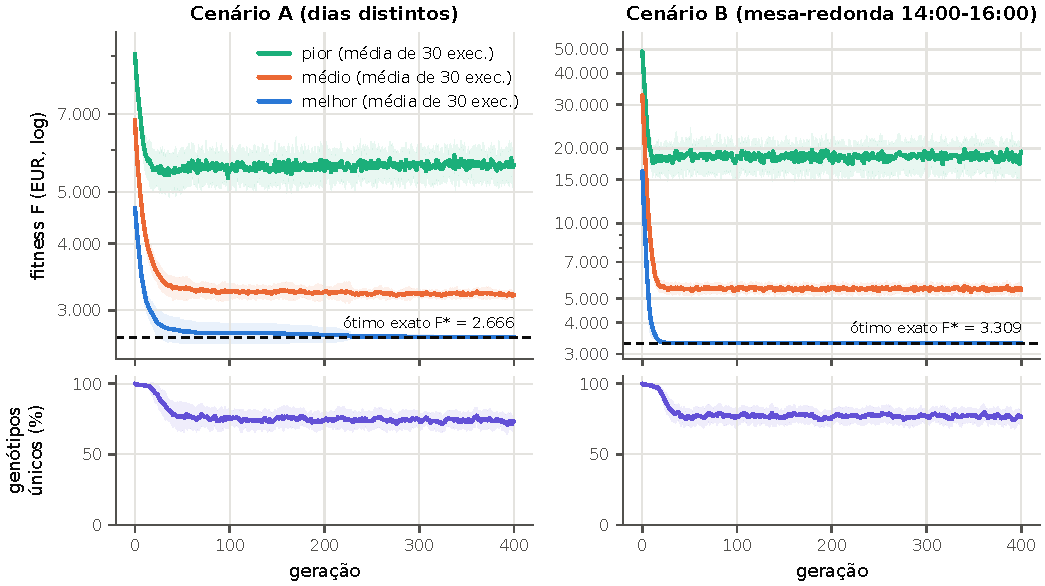
\includegraphics[width=\textwidth]{a1_convergencia.pdf}
\caption{Atividade 1: fitness melhor, médio e pior da população por geração (média de 30 execuções; faixa $=\pm1$ desvio padrão; eixo logarítmico) e fração de genótipos distintos na população. A linha tracejada é o ótimo exato $F^*$.}
\label{fig:a1_conv}
\end{figure*}

\textbf{Convergência e estatísticas.} A Fig.~\ref{fig:a1_conv} e a Tabela~\ref{tab:a1_stats} mostram os resultados. No cenário~A, a média do melhor $F$ foi 2.674,0~EUR (desvio padrão 18,2; variância 331,0), contra $F^*=2.666$. O AG atingiu o ótimo exato em 25 das 30 execuções, em média na geração 125 (mediana 79). As cinco restantes convergiram para o mesmo ótimo local, $F=2.714$ (gap de 1,8\%). Nele, os voos de ida coincidem com os do ótimo, mas o bloco de volta está cerca de dois voos mais cedo (07:50--09:49). Deslocar esse bloco em uma posição leva a $F=3.083$, então nem a mutação de bloco atravessa essa barreira com facilidade. No cenário~B, todas as 30 execuções atingiram $F^*=3.309$, com variância nula, em média na geração 21. A janela da mesa-redonda reduz muito a região factível, e a penalidade proporcional conduz a população até ela já nas primeiras gerações. O pior indivíduo e a média da população permanecem altos durante toda a execução, porque as mutações mantêm diversidade: cerca de 75\% dos genótipos continuam distintos. Esse é o comportamento esperado com elitismo e mutação ativos. A busca aleatória com o mesmo orçamento de 58.150 avaliações ficou muito longe do ótimo: em média 3.718,5 no cenário~A e 8.602,1 no cenário~B (Fig.~\ref{fig:a1_dist}).

\begin{figure}[!t]
\centering
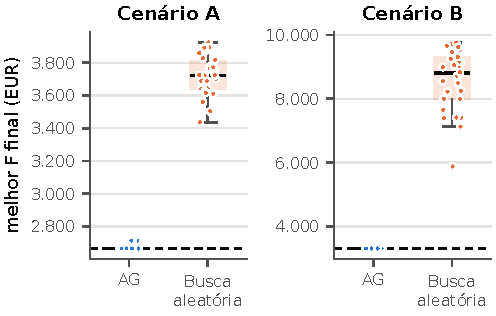
\includegraphics[width=\columnwidth]{a1_distribuicao_final.pdf}
\caption{Melhor $F$ final em 30 execuções: AG versus busca aleatória com o mesmo número de avaliações. Linha tracejada: ótimo exato.}
\label{fig:a1_dist}
\end{figure}

\textbf{Melhores roteiros.} As Tabelas~\ref{tab:a1_best_A} e~\ref{tab:a1_best_B} e a Fig.~\ref{fig:a1_rot} mostram os melhores roteiros, que coincidem com os ótimos exatos. No cenário~A, as chegadas se concentram entre 14:17 e 15:02, e o grupo espera só 81 minutos no total antes de a van partir. A maior parte da espera (541 min) fica na volta, porque os voos de retorno mais baratos e sincronizados partem entre 10:32 e 12:37, e o grupo é deixado às 09:32. No cenário~B, todos chegam até 10:45 e partem entre 18:17 e 20:27. O custo sobe para 2.415~EUR, já que os voos compatíveis com a janela são mais caros, e a espera na volta cresce porque a van chega a FCO às 16:45, antes de qualquer partida factível.

\begin{table}[!t]
\centering
\footnotesize
\setlength{\tabcolsep}{3.5pt}
\caption{Melhor roteiro encontrado pelo AG -- cenário A (ida e volta em dias distintos (sem janela)). Esperas em minutos.}
\label{tab:a1_best_A}
\begin{tabular}{@{}lrrrrrr@{}}
\toprule
Origem & Ida & EUR & Esp. & Volta & EUR & Esp. \\
\midrule
LIS & 12:18--14:56 & 172 & 6 & 11:07--13:24 & 171 & 95 \\
MAD & 12:44--14:17 & 134 & 45 & 10:33--13:11 & 132 & 61 \\
CDG & 11:28--14:40 & 248 & 22 & 12:37--15:05 & 170 & 185 \\
DUB & 12:34--15:02 & 109 & 0 & 10:33--12:03 & 74 & 61 \\
BRU & 10:30--14:57 & 290 & 5 & 10:51--14:16 & 256 & 79 \\
LHR & 12:08--14:59 & 149 & 3 & 10:32--13:16 & 139 & 60 \\
\midrule
Total &  & 1.102 & 81 &  & 942 & 541 \\
\bottomrule
\end{tabular}
\par\smallskip\parbox{0.95\linewidth}{\scriptsize Van sai de FCO às 15:02 e deixa o grupo em FCO às 09:32. Custo = 2.044 EUR; espera = 622 min; $F$ = 2.666.}
\end{table}

% Arquivo gerado automaticamente por src/ -- nao editar manualmente.
\begin{table}[!t]
\centering
\footnotesize
\setlength{\tabcolsep}{3.5pt}
\caption{Melhor roteiro encontrado pelo AG -- cenário B (mesa-redonda no mesmo dia (14:00-16:00)). Esperas em minutos.}
\label{tab:a1_best_B}
\begin{tabular}{@{}lrrrrrr@{}}
\toprule
Origem & Ida & EUR & Esp. & Volta & EUR & Esp. \\
\midrule
LIS & 07:39--10:24 & 219 & 21 & 18:25--20:34 & 205 & 100 \\
MAD & 08:25--10:34 & 157 & 11 & 18:33--20:22 & 143 & 108 \\
CDG & 07:34--09:40 & 324 & 65 & 20:27--23:42 & 169 & 222 \\
DUB & 08:04--10:11 & 95 & 34 & 18:24--20:49 & 124 & 99 \\
BRU & 06:12--10:22 & 230 & 23 & 18:44--22:42 & 351 & 119 \\
LHR & 08:27--10:45 & 139 & 0 & 18:17--21:04 & 259 & 92 \\
\midrule
Total &  & 1.164 & 154 &  & 1.251 & 740 \\
\bottomrule
\end{tabular}
\par\smallskip\parbox{0.95\linewidth}{\scriptsize Van sai de FCO às 10:45 e deixa o grupo em FCO às 16:45. Custo = 2.415 EUR; espera = 894 min; $F$ = 3.309.}
\end{table}


\begin{figure*}[!t]
\centering
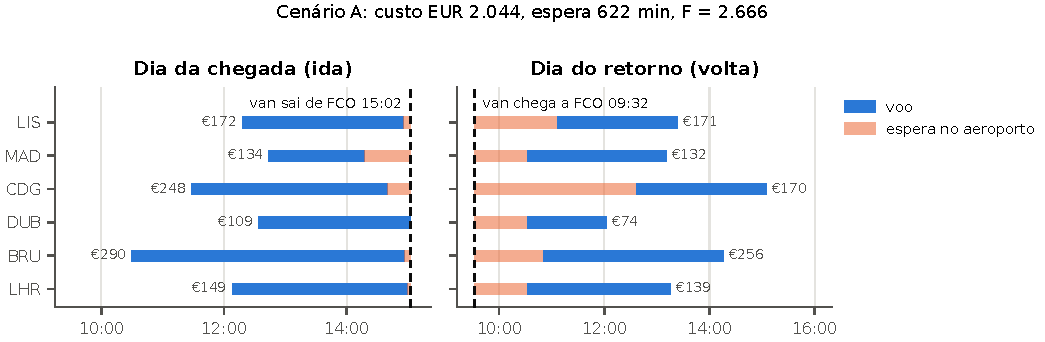
\includegraphics[width=0.93\textwidth]{a1_roteiro_A.pdf}\\[2pt]
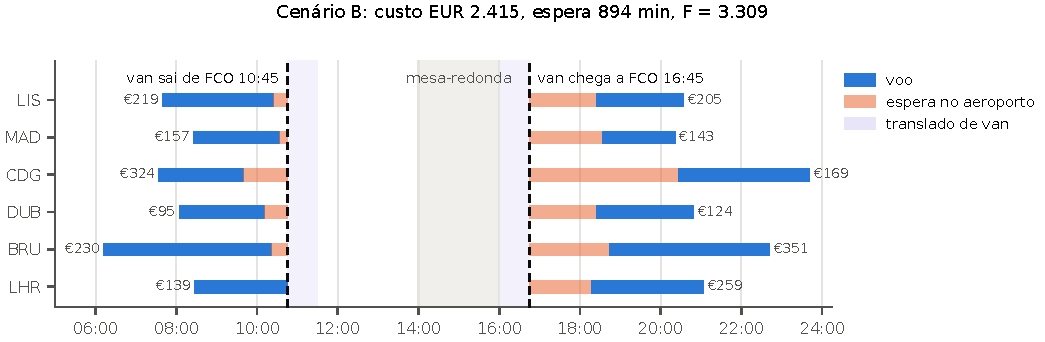
\includegraphics[width=0.93\textwidth]{a1_roteiro_B.pdf}
\caption{Roteiros ótimos encontrados pelo AG. Barras azuis: voos (preço à margem). Barras laranja: espera em FCO. Linhas tracejadas: partida e chegada da van. No cenário B, a faixa cinza é a mesa-redonda e as faixas lilás são os translados.}
\label{fig:a1_rot}
\end{figure*}

\textbf{Sensibilidade.} A Tabela~\ref{tab:a1_sens} varia um parâmetro por vez no cenário~A, o mais difícil. Os efeitos mais fortes vêm da mutação de bloco e do elitismo:
\begin{itemize}
  \item Sem mutação de bloco ($p_{\text{shift}}=0$), o AG atinge o ótimo em apenas 7/30 execuções, com média 2.840. A diferença em relação à base (25/30) é significativa: $p\approx6\times10^{-6}$ no teste exato de Fisher. A estagnação descrita na Seção~\ref{sec:a1} confirma-se.
  \item Sem elitismo ($e=0$), a taxa cai para 2/30, porque as boas soluções se perdem entre gerações.
  \item Um torneio grande ($k=5$) ou $p_m$ alto ($0{,}10$) também pioram o resultado: o primeiro aumenta a pressão seletiva e causa convergência prematura; o segundo destrói os grupos sincronizados.
\end{itemize}
Algumas variações ($p_{\text{shift}}=0{,}5$, $p_c=0{,}6$, $e=10$, $N=300$) ficaram ligeiramente acima da base. As diferenças, porém, são de poucas execuções em 30. Por exemplo, 29/30 contra 25/30 dá $p\approx0{,}19$ no teste exato de Fisher, ou seja, a diferença não é significativa. Por isso a configuração base, definida \emph{antes} com outras seeds, foi mantida.

% Arquivo gerado automaticamente por src/ -- nao editar manualmente.
\begin{table}[!t]
\centering
\footnotesize
\setlength{\tabcolsep}{4pt}
\caption{Análise de sensibilidade (um fator por vez) no cenário A. Em negrito, o valor da configuração base.}
\label{tab:a1_sens}
\begin{tabular}{@{}llrrrr@{}}
\toprule
Fator & Valor & Média $F$ & DP & Sucesso & Ger. \\
\midrule
Torneio $k$ & 2 & 2.688{,}5 & 24{,}3 & 15/30 & 136 \\
 & \textbf{3} & 2.674{,}0 & 18{,}2 & 25/30 & 125 \\
 & 5 & 2.704{,}6 & 90{,}3 & 17/30 & 74 \\
\midrule
Cruzamento & 1 ponto & 2.720{,}4 & 130{,}9 & 20/30 & 96 \\
 & 2 pontos & 2.708{,}0 & 125{,}7 & 26/30 & 79 \\
 & \textbf{uniforme} & 2.674{,}0 & 18{,}2 & 25/30 & 125 \\
\midrule
$p_c$ & 0{,}60 & 2.672{,}5 & 27{,}8 & 28/30 & 139 \\
 & \textbf{0{,}90} & 2.674{,}0 & 18{,}2 & 25/30 & 125 \\
 & 1{,}00 & 2.735{,}7 & 150{,}5 & 19/30 & 142 \\
\midrule
$p_m$ (gene) & 0{,}02 & 2.701{,}5 & 122{,}5 & 26/30 & 98 \\
 & \textbf{0{,}05} & 2.674{,}0 & 18{,}2 & 25/30 & 125 \\
 & 0{,}10 & 2.716{,}9 & 113{,}2 & 14/30 & 98 \\
\midrule
$p_{\mathrm{shift}}$ & 0{,}00 & 2.840{,}0 & 155{,}0 & 7/30 & 42 \\
 & 0{,}10 & 2.750{,}2 & 155{,}2 & 14/30 & 146 \\
 & \textbf{0{,}30} & 2.674{,}0 & 18{,}2 & 25/30 & 125 \\
 & 0{,}50 & 2.666{,}1 & 0{,}5 & 29/30 & 107 \\
\midrule
Elitismo $e$ & 0 & 2.826{,}5 & 163{,}4 & 2/30 & 81 \\
 & 1 & 2.719{,}2 & 123{,}5 & 18/30 & 138 \\
 & \textbf{5} & 2.674{,}0 & 18{,}2 & 25/30 & 125 \\
 & 10 & 2.683{,}7 & 88{,}5 & 28/30 & 96 \\
\midrule
População $N$ & 50 & 2.764{,}0 & 155{,}5 & 11/30 & 116 \\
 & \textbf{150} & 2.674{,}0 & 18{,}2 & 25/30 & 125 \\
 & 300 & 2.679{,}8 & 47{,}2 & 27/30 & 132 \\
\bottomrule
\end{tabular}
\par\smallskip\parbox{0.95\linewidth}{\scriptsize Sucesso: execuções que atingiram o ótimo exato. Ger.: geração média em que $F^*$ foi atingido.}
\end{table}


\textbf{Compromisso custo $\times$ espera.} A Fig.~\ref{fig:a1_pareto} varia $\lambda$ entre 0 e 4~EUR/min (10 execuções por valor) e compara as soluções do AG com a fronteira de Pareto exata. Com $\lambda=0$ otimiza-se apenas o preço: no cenário A, o custo mínimo é 1.566~EUR, com 4.329~min de espera. Com $\lambda\ge2$ prioriza-se a espera: 533~min, a 2.136~EUR. O valor $\lambda=1$ escolhe um ponto intermediário (2.044~EUR e 622~min). As soluções do AG ficam próximas da fronteira e longe da nuvem de soluções aleatórias, mas a taxa de acerto do ótimo de $F_\lambda$ depende de $\lambda$:
\begin{itemize}
  \item no cenário~B, o AG acertou 60 de 60 execuções, com gap nulo;
  \item no cenário~A, acertou 10/10 com $\lambda=0$, caso em que o problema se reduz a escolher o voo mais barato de cada rota, de forma independente; com $\lambda=1$, acertou 7/10, com gap médio de 0,5\%;
  \item ainda no cenário~A, acertou só 0/10 com $\lambda=0{,}25$ (gap médio 2,9\%) e 4/10 com $\lambda=4$ (gap médio 7,5\%, máximo 19\%).
\end{itemize}
O termo de espera é o que acopla os genes pelo $\max$ e pelo $\min$. Mudar $\lambda$ altera o equilíbrio entre esse termo e o preço e, com ele, a posição dos ótimos locais. Como os parâmetros foram ajustados para $\lambda=1$, outros valores de $\lambda$ pedem um novo ajuste, por exemplo um $p_{\text{shift}}$ ou um $G$ maiores. A fitness escalar com $\lambda$ explícito continua sendo uma forma transparente de expor ao usuário a troca entre os dois objetivos.

\begin{figure*}[!t]
\centering
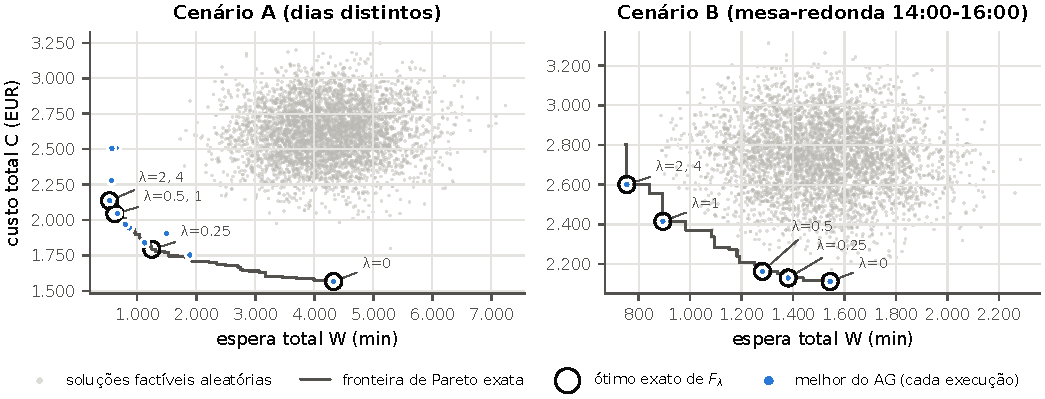
\includegraphics[width=\textwidth]{a1_custo_vs_espera.pdf}
\caption{Custo total $\times$ espera total. Cinza: 4.000 soluções factíveis aleatórias. Linha: fronteira de Pareto exata. Círculos: ótimo exato de $F_\lambda=C+\lambda W$ para $\lambda\in\{0;0{,}25;0{,}5;1;2;4\}$. Pontos azuis: melhor solução de cada execução do AG.}
\label{fig:a1_pareto}
\end{figure*}

% ----------------------------------------------------------------------------
\subsection{Atividade 2}
\label{sec:res_a2}
\begin{table}[!t]
\centering
\footnotesize
\setlength{\tabcolsep}{4pt}
\caption{Estatísticas do melhor valor final de $f$ na Atividade 2.}
\label{tab:a2_stats}
\begin{tabular}{@{}lrr@{}}
\toprule
Métrica (30 execuções) & $n=2$ & $n=10$ \\
\midrule
Média do melhor $f$ & $1{,}85\times10^{-5}$ & $5{,}35\times10^{-5}$ \\
Variância & $1{,}22\times10^{-9}$ & $1{,}85\times10^{-9}$ \\
Desvio padrão & $3{,}50\times10^{-5}$ & $4{,}30\times10^{-5}$ \\
Mínimo & $4{,}78\times10^{-8}$ & $9{,}30\times10^{-6}$ \\
Mediana & $7{,}34\times10^{-6}$ & $4{,}68\times10^{-5}$ \\
Máximo & $1{,}50\times10^{-4}$ & $1{,}95\times10^{-4}$ \\
Média de $\log_{10} f$ ($\pm$ DP) & $-5{,}25 \pm 0{,}76$ & $-4{,}40 \pm 0{,}35$ \\
$\|\mathbf{x}_{best}\|$ médio & $2{,}33\times10^{-4}$ & $4{,}84\times10^{-4}$ \\
Execuções com $f<0{,}5$ (bacia global) & 30/30 & 30/30 \\
Execuções com $f<10^{-4}$ & 28/30 & 28/30 \\
Geração p/ $f<10^{-4}$ (média) & 47{,}2 & 403{,}6 \\
$\bar f$ da pop. final (média) & 11{,}569 & 12{,}846 \\
Tempo por execução (s) & 0{,}15 & 1{,}82 \\
\midrule
Busca aleatória: média & 0{,}394 & 57{,}098 \\
Busca aleatória: desvio padrão & 0{,}259 & 5{,}307 \\
\bottomrule
\end{tabular}
\par\smallskip\parbox{0.95\linewidth}{\scriptsize Variância e desvio padrão amostrais. A busca aleatória usa o número máximo de avaliações do AG.}
\end{table}


\begin{figure*}[!t]
\centering
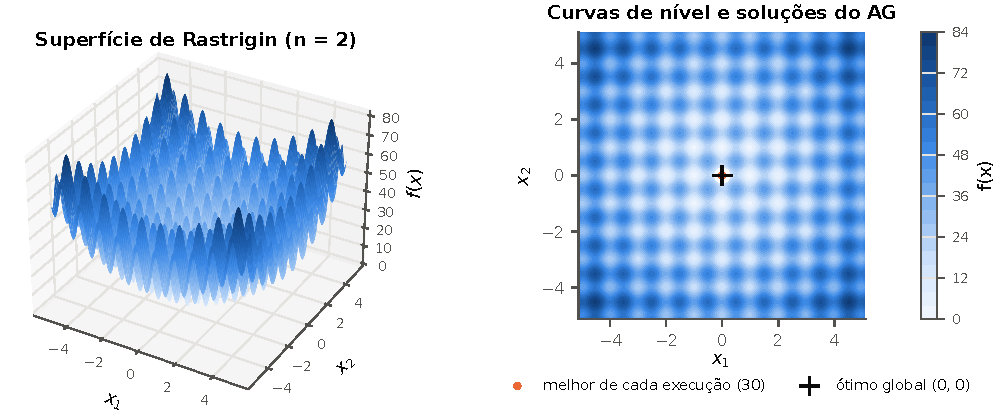
\includegraphics[width=0.88\textwidth]{a2_superficie.pdf}
\caption{Função de Rastrigin para $n=2$: superfície (esquerda) e curvas de nível com a melhor solução de cada uma das 30 execuções (direita), todas sobre o ótimo global.}
\label{fig:a2_surf}
\end{figure*}

\begin{figure*}[!t]
\centering
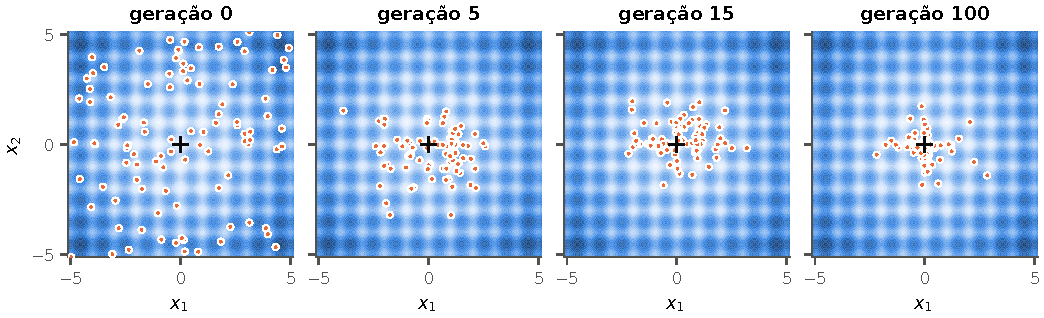
\includegraphics[width=\textwidth]{a2_populacao_n2.pdf}
\caption{População de uma execução ($n=2$, seed 2026) nas gerações 0, 5, 15 e 100. A população se concentra rapidamente na bacia central.}
\label{fig:a2_pop}
\end{figure*}

\begin{figure*}[!t]
\centering
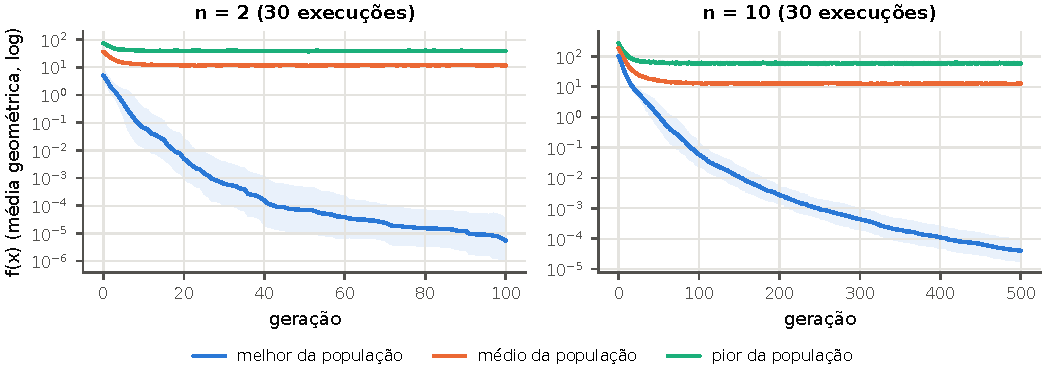
\includegraphics[width=\textwidth]{a2_convergencia.pdf}
\caption{Atividade 2: $f$ melhor, médio e pior da população por geração (média geométrica de 30 execuções; faixa $=\pm1$ desvio padrão em escala logarítmica).}
\label{fig:a2_conv}
\end{figure*}

\textbf{Convergência.} A Tabela~\ref{tab:a2_stats} e as Figs.~\ref{fig:a2_surf}--\ref{fig:a2_dist} resumem os resultados.
\begin{itemize}
  \item \textbf{$n=2$:} a população chega à bacia global ($f<0{,}5$) em média na geração 6,9, e as 30 execuções terminam a uma distância média de $2{,}3\times10^{-4}$ da origem. A média do melhor $f$ final foi $1{,}85\times10^{-5}$, com desvio padrão de $3{,}50\times10^{-5}$ e variância de $1{,}22\times10^{-9}$. Em 28 das 30 execuções, $f<10^{-4}$.
  \item \textbf{$n=10$:} a entrada na bacia global ocorre em média na geração 63,7. A média final foi $5{,}35\times10^{-5}$, com desvio padrão de $4{,}30\times10^{-5}$ e variância de $1{,}85\times10^{-9}$. Também aqui as 30 execuções terminam na bacia global, e 28/30 abaixo de $10^{-4}$.
\end{itemize}
Depois de encontrar a bacia, a curva do melhor (Fig.~\ref{fig:a2_conv}) cai de forma aproximadamente log-linear. É a fase de refinamento, conduzida pela mutação polinomial e pelo SBX com índices de distribuição altos. As curvas do médio e do pior se estabilizam em torno de $f\approx12$, porque a mutação continua lançando indivíduos em bacias vizinhas: é o custo de manter a exploração. A busca aleatória com o mesmo orçamento obteve médias de 0,394 ($n=2$) e 57,1 ($n=10$). Em 10 dimensões, a amostragem uniforme praticamente não avança, e a diferença para o AG é de seis ordens de grandeza.

\textbf{Sensibilidade.} A Tabela~\ref{tab:a2_sens} ($n=10$) mostra um comportamento oposto ao da Atividade~1: mais pressão seletiva e mais elitismo \emph{melhoram} a precisão. Com $k=5$, a média foi $3{,}4\times10^{-10}$; com $e=10$, $2{,}8\times10^{-9}$. Por outro lado, $k=2$ e $e=0$ pioram o resultado, e uma mutação excessiva ($p_{\text{gene}}=0{,}2$) tirou 4 das 30 execuções da bacia global. A explicação é que a Rastrigin é separável e o SBX atua coordenada a coordenada, então a população encontra a bacia global com facilidade, e o gargalo passa a ser o refinamento local, que se beneficia de explotação. Pela mesma razão, uma mutação mais concentrada ($\eta_m=50$) e menos frequente ($p_{\text{gene}}=0{,}05$) também ajudou. Na Atividade~1, ao contrário, a dificuldade era escapar de ótimos locais enganosos, e a diversidade foi decisiva. Os resultados sugerem que a configuração base é conservadora para $n=10$; não se verificou se isso se mantém em dimensões maiores.

\begin{figure}[!t]
\centering
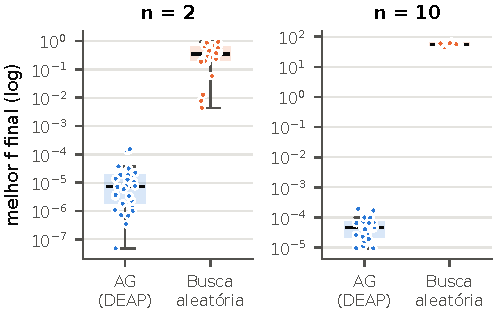
\includegraphics[width=\columnwidth]{a2_distribuicao_final.pdf}
\caption{Melhor $f$ final (escala log) em 30 execuções: AG com DEAP versus busca aleatória com o mesmo número máximo de avaliações.}
\label{fig:a2_dist}
\end{figure}

% Arquivo gerado automaticamente por src/ -- nao editar manualmente.
\begin{table}[!t]
\centering
\footnotesize
\setlength{\tabcolsep}{3pt}
\caption{Sensibilidade dos parâmetros do AG/DEAP na Rastrigin com $n=10$ (um fator por vez; base em negrito).}
\label{tab:a2_sens}
\begin{tabular}{@{}llrrrr@{}}
\toprule
Fator & Valor & Média $f$ & Mediana $f$ & $f<0{,}5$ & $f<10^{-4}$ \\
\midrule
Torneio $k$ & 2 & $2{,}26\times10^{-2}$ & $1{,}70\times10^{-2}$ & 30/30 & 0/30 \\
 & \textbf{3} & $5{,}35\times10^{-5}$ & $4{,}68\times10^{-5}$ & 30/30 & 28/30 \\
 & 5 & $3{,}39\times10^{-10}$ & $1{,}64\times10^{-10}$ & 30/30 & 30/30 \\
\midrule
$p_c$ & 0{,}60 & $2{,}64\times10^{-5}$ & $1{,}56\times10^{-5}$ & 30/30 & 30/30 \\
 & \textbf{0{,}90} & $5{,}35\times10^{-5}$ & $4{,}68\times10^{-5}$ & 30/30 & 28/30 \\
 & 1{,}00 & $5{,}75\times10^{-5}$ & $4{,}11\times10^{-5}$ & 30/30 & 26/30 \\
\midrule
$p_{\mathrm{gene}}$ & 0{,}05 & $7{,}22\times10^{-10}$ & $5{,}14\times10^{-10}$ & 30/30 & 30/30 \\
 & \textbf{0{,}10} & $5{,}35\times10^{-5}$ & $4{,}68\times10^{-5}$ & 30/30 & 28/30 \\
 & 0{,}20 & $2{,}84\times10^{-1}$ & $2{,}01\times10^{-1}$ & 26/30 & 0/30 \\
\midrule
$\eta_m$ & 5{,}00 & $3{,}27\times10^{-4}$ & $2{,}50\times10^{-4}$ & 30/30 & 1/30 \\
 & \textbf{20{,}00} & $5{,}35\times10^{-5}$ & $4{,}68\times10^{-5}$ & 30/30 & 28/30 \\
 & 50{,}00 & $1{,}44\times10^{-5}$ & $1{,}17\times10^{-5}$ & 30/30 & 30/30 \\
\midrule
Elitismo $e$ & 0 & $1{,}05\times10^{-1}$ & $1{,}01\times10^{-1}$ & 30/30 & 0/30 \\
 & \textbf{2} & $5{,}35\times10^{-5}$ & $4{,}68\times10^{-5}$ & 30/30 & 28/30 \\
 & 10 & $2{,}84\times10^{-9}$ & $8{,}30\times10^{-10}$ & 30/30 & 30/30 \\
\bottomrule
\end{tabular}
\end{table}


% ============================================================================
\section{Discussão}
% ============================================================================
\textbf{Representação e operadores.} Nos dois problemas, a representação determinou o desenho dos operadores. Na Atividade~1, a codificação por índices garante validade por construção e dispensa qualquer reparo. A ordenação dos voos por horário, por sua vez, deu sentido às mutações \emph{creep} e de bloco. Na Atividade~2, a representação real com operadores limitados manteve as soluções no domínio, e a natureza coordenada a coordenada do SBX e da mutação polinomial combina com a separabilidade da Rastrigin.

\textbf{Limitações.}
\begin{itemize}
  \item A fitness da Atividade~1 depende das premissas da Seção~\ref{sec:a1_premissas}: uma van única, translado e check-in fixos, e a janela do cenário B. Outras premissas, como permitir duas viagens de van, mudam o problema.
  \item O valor de $\lambda$ é uma escolha de preferência. A Fig.~\ref{fig:a1_pareto} mostra o efeito dessa escolha, em vez de escondê-la.
  \item A validação pelo ótimo exato só foi possível porque a fitness é separável. Com acoplamentos entre ida e volta, por exemplo um custo de diária de van, o AG continuaria aplicável, mas a enumeração não.
\end{itemize}

% ============================================================================
\section{Conclusões}
% ============================================================================
Foram implementados dois AGs: um do zero, para a escolha de voos de um grupo, e outro com \deap{}, para a função de Rastrigin. Na Atividade~1, a modelagem com 12 genes inteiros e a fitness $F=C+\lambda W+P$ produziram roteiros ótimos e coerentes com as premissas de van, check-in e janela do congresso. A validação contra o ótimo global exato mostrou taxa de acerto de 83\% (25/30) no cenário sem janela e de 100\% no cenário com janela. A análise de sensibilidade evidenciou o papel do elitismo e de um operador de mutação adequado à estrutura do problema. Na Atividade~2, o \deap{} com SBX e mutação polinomial limitados levou todas as execuções à bacia do ótimo global, para $n=2$ e para $n=10$. Nos dois problemas, o AG superou com folga a busca aleatória de mesmo orçamento; na Rastrigin com $n=10$, por seis ordens de grandeza.

Como trabalhos futuros, propõem-se:
\begin{itemize}
  \item tratar a Atividade~1 como problema multiobjetivo, com NSGA-II, para obter a fronteira de Pareto em uma única execução;
  \item incluir acoplamentos entre ida e volta e restrições por pesquisador;
  \item avaliar a Rastrigin em dimensões maiores ($n\ge30$).
\end{itemize}

\section*{Disponibilidade do código}
Todo o código, os dados, os resultados brutos (CSV/JSON) e os scripts que geram as figuras e as tabelas acompanham este artigo. A reprodução completa é feita com \code{python executar\_tudo.py} (ver \code{README.md}).

\bibliographystyle{IEEEtran}
\bibliography{referencias}

\end{document}
